\documentclass[11pt,twoside]{article}
\usepackage{etex}
\newcommand{\num}{6{}}

\raggedbottom

%geometry (sets margin) and other useful packages
\usepackage{geometry}
\geometry{top=1in, left=1.4in,right=1.4in,bottom=1in}
 \usepackage{graphicx,booktabs,calc}
\usepackage{float}
\usepackage[table,xcdraw]{xcolor}
\usepackage{multirow}
\usepackage{rotating,tabularx}

%=== GRAPHICS PATH ===========
\graphicspath{{./images/}}
% Marginpar width
%Marginpar width
\newcommand{\pts}[1]{\marginpar{\small\hspace{0pt} \textit{[#1]} } }
\setlength{\marginparwidth}{1in}
%\reversemarginpar
%\setlength{\marginparsep}{.02in}

%% Fonts
% \usepackage{fourier}
% \usepackage[T1]{pbsi}

\usepackage{lmodern}
\usepackage[T1]{fontenc}
%\usepackage{minted}

\usepackage{rotating}

\usepackage{marginnote}

\usepackage{soul} % for highlighting, striking out, etc
\setstcolor{red}

%% Cite Title
\usepackage[style=authoryear,natbib,maxcitenames=2,doi=false,isbn=false,url=false,eprint=false,uniquename=false]{biblatex}
\addbibresource{../network-resilience.bib}
\addbibresource{../bems-references.bib}

%%% Counters
\usepackage{chngcntr,mathtools}
\counterwithout{figure}{section}
\counterwithout{table}{section}

\numberwithin{equation}{section}

%% Captions
\usepackage{caption}
\captionsetup{
  labelsep=quad,
  justification=raggedright,
  labelfont=sc
}

%AMS-TeX packages
\usepackage{amssymb,amsmath,amsthm}
\usepackage{bm}
\usepackage[mathscr]{eucal}
\usepackage{colortbl}
\usepackage{color}


\usepackage{epstopdf,subfigure,hyperref,enumerate,polynom,polynomial}
\usepackage{multirow,minitoc,fancybox,array,multicol}

\definecolor{slblue}{rgb}{0,.3,.62}
\hypersetup{
    colorlinks,%
    citecolor=blue,%
    filecolor=blue,%
    linkcolor=blue,
    urlcolor=slblue
}

%%%TIKZ
\usepackage{tikz}
\usepackage{pgfplots}
\usepackage{pgfplotstable}
\usepackage{pgfgantt}
\pgfplotsset{compat=newest}

\usetikzlibrary{arrows,shapes,positioning}
\usetikzlibrary{decorations.markings}
\usetikzlibrary{shadows,automata}
\usetikzlibrary{patterns}
%\usetikzlibrary{circuits.ee.IEC}
\usetikzlibrary{decorations.text}
% For Sagnac Picture
\usetikzlibrary{%
    decorations.pathreplacing,%
    decorations.pathmorphing%
}

%
%Redefining sections as problems
%
\makeatletter
\newenvironment{question}{\@startsection
	{section}
	{1}
	{-.2em}
	{-3.5ex plus -1ex minus -.2ex}
    	{1.3ex plus .2ex}
    	{\pagebreak[3]%forces pagebreak when space is small; use \eject for better results
	\large\bf\noindent{Question }
	}
	}
	%{\vspace{1ex}\begin{center} \rule{0.3\linewidth}{.3pt}\end{center}}
	%\begin{center}\large\bf \ldots\ldots\ldots\end{center}}
\makeatother

%
%Fancy-header package to modify header/page numbering
%
%\renewcommand{\chaptermark}[1]{ \markboth{#1}{} }
\renewcommand{\sectionmark}[1]{ \markright{#1}{} }

\usepackage{fancyhdr}
%\pagestyle{fancy}
%\addtolength{\headwidth}{\marginparsep} %these change header-rule width
%\addtolength{\headwidth}{\marginparwidth}
%\fancyheadoffset{30pt}
%\fancyfootoffset{30pt}
%\fancyhead[LO,RE]{\small  \it \nouppercase{\leftmark}}
%\fancyhead[RO,LE]{\small Page \thepage}
%\fancyfoot[RO,LE]{\small }% PR \num S-2015}
%\fancyfoot[LO,RE]{\small }%\scshape MODL}
%\cfoot{}
\renewcommand{\headrulewidth}{0.1pt}
\renewcommand{\footrulewidth}{0pt}
%\setlength\voffset{-0.25in}
%\setlength\textheight{648pt}


\usepackage{paralist}


%%% FORMAT PYTHON CODE
\usepackage{listings}
% Default fixed font does not support bold face
\DeclareFixedFont{\ttb}{T1}{txtt}{bx}{n}{8} % for bold
\DeclareFixedFont{\ttm}{T1}{txtt}{m}{n}{8}  % for normal

% Custom colors
\usepackage{color}
\definecolor{deepblue}{rgb}{0,0,0.5}
\definecolor{deepred}{rgb}{0.6,0,0}
\definecolor{deepgreen}{rgb}{0,0.5,0}

%\usepackage{listings}

% % Python style for highlighting
% \newcommand\pythonstyle{\lstset{
% language=Python,
% basicstyle=\footnotesize\ttm,
% otherkeywords={self},             % Add keywords here
% keywordstyle=\footnotesize\ttb\color{deepblue},
% emph={MyClass,__init__},          % Custom highlighting
% emphstyle=\footnotesize\ttb\color{deepred},    % Custom highlighting style
% stringstyle=\color{deepgreen},
% frame=tb,                         % Any extra options here
% showstringspaces=false            %
% }}

% % Python environment
% \lstnewenvironment{python}[1][]
% {
% \pythonstyle
% \lstset{#1}
% }
% {}

% % Python for external files
% \newcommand\pythonexternal[2][]{{
% \pythonstyle
% \lstinputlisting[#1]{#2}}}

% % Python for inline
% \newcommand\pythoninline[1]{{\pythonstyle\lstinline!#1!}}


\newcommand{\osn}{\oldstylenums}
\newcommand{\dg}{^{\circ}}
\newcommand{\lt}{\left}
\newcommand{\rt}{\right}
\newcommand{\pt}{\phantom}
\newcommand{\tf}{\therefore}
\newcommand{\?}{\stackrel{?}{=}}
\newcommand{\fr}{\frac}
\newcommand{\dfr}{\dfrac}
%\newcommand{\ul}{\underline}
\newcommand{\tn}{\tabularnewline}
\newcommand{\nl}{\newline}
\newcommand\relph[1]{\mathrel{\phantom{#1}}}
\newcommand{\cm}{\checkmark}
\newcommand{\ol}{\overline}
\newcommand{\rd}{\color{red}}
\newcommand{\bl}{\color{blue}}
\newcommand{\pl}{\color{purple}}
\newcommand{\og}{\color{orange!90!black}}
\newcommand{\gr}{\color{green!40!black}}
\newcommand{\nin}{\noindent}
\newcommand{\la}{\lambda}
\renewcommand{\th}{\theta}
\newcommand{\al}{\alpha}
\newcommand{\G}{\Gamma}
\newcommand*\circled[1]{\tikz[baseline=(char.base)]{
            \node[shape=circle,draw,thick,inner sep=1pt] (char) {\small #1};}}

\newcommand{\bc}{\begin{compactenum}[\quad--]}
\newcommand{\ec}{\end{compactenum}}

\newcommand{\p}{\partial}
\newcommand{\pd}[2]{\frac{\partial{#1}}{\partial{#2}}}
\newcommand{\dpd}[2]{\dfrac{\partial{#1}}{\partial{#2}}}
\newcommand{\pdd}[2]{\frac{\partial^2{#1}}{\partial{#2}^2}}


%%%%%%%%%%%%%%%%%%%%%%%%%%%%%%%%%%%%%%%%%%%%%%%%%%%
%%%%%%%%%%%%%%%%%%%%%%%%%%%%%%%%%%%%%%%%%%%%%%%%%%%

\begin{document}

\title{Multilayer critical infrastructure network modeling for equitable resilience}

\author{}
\date{\today}
\maketitle

%\thispagestyle{empty}

%\tableofcontents

\section{Introduction}
The frequency and magnitude of extreme events have significantly increased all over the globe during the past two decades
\citep{kermanshah2017robustness}. The performance of \st{transportation} critical infrastructure networks can be
seriously affected by these extreme events \citep{ilbeigi2019statistical}.  Transportation systems, in particular, are
vulnerable to a widespread range of natural events and disruptions such as such as hurricanes, tornadoes, earthquakes,
wildfires, traffic incidents, snowing, flooding, infrastructure failures, among others
\citep{bhavathrathan2018algorithm}, \citep{twumasi-boakye2018resilience}.  For example, \citet{ilbeigi2019statistical}
\st{has} developed a quantifying resilience framework for the 2012 Hurricane Sandy, which \st{has} hit urban areas in
New York City and \st{h}was identified as the fourth costliest hurricane in U.S. history.  He has evaluated
transportation dataset for a period of four weeks (two weeks before the hurricane and two weeks after it) and
considering the closeness centrality index, he found out that the New York City transportation network was affected by
the hurricane for 135 hours. The proposed framework helps decision makers to identify more vulnerable parts of the
network, which are more likely to fail first \citep{ilbeigi2019statistical}.
  
In order to develop a more reliable framework for quantifying resilience in our communities, the focus of the
resilience studies should be shifted from transportation network to a more comprehensive view in which all critical
infrastructures elements are included. For instance, one of the most vulnerable elements in road transportation systems
are bridges which can highly affect robustness of the transportation network as a whole
\citep{zhang2017resiliencebased}.  Moreover, 
it is critical to have a resilient transportation network during and after a disaster, to ensure emergency services,
rescue operations, and access to major population and activity centers in a city \citep{ilbeigi2019statistical}.
Although it is very important to make decisions regarding restoration of transportation networks in a short period after
event, these decisions have to be made \st{in a way that} with regard to various decision-making criteria and resource
constraints have been made in to account \citep{liu2020optimal}.  So it is of vital importance for decision makers to
have access to a promising decision making framework able of quantifying transportation network resilience. This way,
they can ensure availability of a promising transportation network with the optimum capacity, when a disaster occurs.

Network analysis has long been considered an effective approach to studying the behavior of complex systems, such as
social, biological and transportation systems. Representing transportation networks through graphs, is one of the
primary steps in quantifying transportation networks, which have been conducted by many resilience studies. There are
different approaches in modelling transportation networks from considering cities as nodes and traffic roads as edges
\citep{ip2009resilience}, and considering potential traffic bottlenecks in a city as nodes and streets as edges
\citep{das2020approach} to considering intersections and state bridges as nodes and interstates, highways or spurs as
edges \citep{antony2017developing}.  Traditional network analyses, however, fail to provide a comprehensive overview of
a complex system, as they ignore the presence of multiple type of edges of a system in which entities have a different
set of neighbors in each layer \citep{domenico2013mathematical}. Focusing on multilayer networks in the field of network
resilience is very important due to the criticality and complexity related to these infrastructures. Transport processes
in a multilayer framework reveal complex interdependencies compared to those in a single layer representation
\citep{wu2020traffic}, yielding important insights for better decision-making.

Moreover, one important criterion, which has been neglected in quantifying critical infrastructure resilience, is social
equity. People’s vulnerability is affected by their exposure to hazards and their ability to avoid or manage the effects
of the hazard \citep{cutter1995race}.  Studies have shown that class, race and ethnicity, gender, disability, political
power, personal wealth, age, housing ownership and occupation can affect vulnerability against hazards
\citep{bolin2018race, cutter1995race}. Although there are many studies that consider social equity in planning
transportation networks, there is a significant gap in including social equity as an important factor in developing
resilience approaches in the overall critical infrastructure systems of a community and their interdependencies.  Given
that these systems as the main foundation for national security, economy, public welfare and individuals’ daily
activities \citep{qiang2019empirical}, it is critical to develop a comprehensive quantifying framework for network
resilience. Although previous studies provide valuable insights about transportation network resilience, there is an
urgent need to broaden this concept by considering equity metrics and also by encompassing critical infrastructure
systems including bridges, buildings, etc as a multilayered network to develop a decision making framework for
restoration of a transportation infrastructure in case of a disaster.

\section{Network resilience modeling}

Recently, the focus of transport infrastructure management has switched from protection to resilience
\citep{das2020approach}. Moreover, as a result of the developments in resilience engineering studies, the definition of
system resilience has shifted from a system's ability to deal with threats to a system's ability to adjust its
functionality \citep{hollnagel2010resilience}.  Based on this new definition, a system is resilient when it can respond
to what happens, monitor critical developments, anticipate future threats and sustain required functions
\citep{hollnagel2010resilience}. More formally, the resilience of a network or system refers to its capability to
withstand, adapt to and recover fully or partially after a disruptive event \citep{aydin2018framework},
\citep{almoghathawi2019component}, which can be natural or man-made \citep{ahmed2020resilience}.
\citet{weilant2019incorporating} have suggested three different aspects associated with the concept of resilience:
\begin{itemize}
  \item Decreasing the probability of a disaster and increasing the ability of a community to resist a disaster
  \item Increasing the adaptability of a system while maintaining functions in the presence of a disaster
  \item Decreasing the needed time for the system to recovery
to normal functioning
\end{itemize}
Ten dimensions of resilience in transportation systems have been identified. These dimensions are redundancy, diversity,
efficiency, components' dependency, strength, stakeholders' collaboration \citep{ahmed2020resilience}, adaptability,
mobility performance, safety performance, and the ability to recover quickly \citep{ahmed2020resilience},
\citep{murray-tuite2006comparison}.


\subsection{Modeling approaches}
Critical infrastructure are those that if destroyed or rendered unavailable will significantly impact social or economic
welfare or affect national security, national public health or safety. \citep{skrlj2019py3plex}. Having a resilient
critical infrastructure is vital for a society in order to resist, respond to, and recover from disruptive events
\citep{tingting2020transportation}. Transportation infrastructure has been identified as one of critical infrastructure
systems essential to the well-being of modern societies \citep{zhang2016resiliencebased}.

Research on transportation system resilience began in the 1990s \citep{ahmed2020resilience}. Since the concept of
resilience engineering has emerged, different related concepts and methods has been addressed by many scholars and most
of the studies on transportation system resilience studies focused on the resilience of the roadway-based transportation
system \citep{ahmed2020resilience}. At the beginning of this journey, most of the studies focused on providing
qualitative overview of resilience \citep{baroud2014inherent}, \citep{bhatia2015network} but providing a quantitative
overview of resilience is attracting more attention during past years and several quantifying framework for
transportation networks resilience have been proposed by scholars \citep{adjetey-bahun2014simulationbased},
\citep{cavallaro2014assessment}, \citep{bhatia2015network}, \citep{donovan2017empirically}.

Network system resilience can be modelled considering two phases: pre-disaster phase and post-disaster phase
\citep{ahmed2020resilience}. Some studies have further categorized the post-disaster phase into two sub-phases: response
and restoration. The response phase is shortly after the disruptive event and restoration phase follows the response
phase. During restoration phase the infrastructure is waiting for repair, but daily travel demand has recovered to a
relatively normal level, although some demand cannot be satisfied by the degraded infrastructure network
\citep{tingting2020transportation}. Optimal recovery strategies to a disaster within a given network may differ by
hazard, community /cluster/neighborhood or objective \citep{bhatia2015network}. So it is critical to develop a decision
making framework, which is capable of reflecting changes per phases and modifying itself based on the situation. As a
result, developing a dynamic model, which considers multiple efficient measures for quantifying resilience and the
effect of different kinds of disasters from mild to sever, becomes more and more important.

In order to come up with an efficient model, it is critical to evaluate all relevant historical data. With increasing
availability of data, machine learning technique is applying in many areas.  Machine learning is a technique to predict
the behaviour of a system based on an analytical model build upon learning from the latest patterns of historical data
\citep{tizghadam2019machine}.  One of the most prevalent application of machine learning techniques, is in time
prediction based on current and past data. A significant number of studies have focused on predicting future delays in
transportation networks \citep{chandramouleeswaran2018machine, takeichi2017prediction, choi2016prediction}.

Machine learning is also applied in many other areas such as smart transportation, intelligent transportation networks,
car sharing placement, public transport locationing \citep{tizghadam2019machine}, traffic assignment, predicting
behavior of an individual driver in various traffic flow conditions, providing driving decision algorithm for
self-driving cars and predicting speed in roadways \citep{bhavsar2017chapter}.  Machine learning techniques have also
been employed toward system resilience. For example, there is a study that focus on estimating clearance time after an
incident is investigated \citep{tang2020statistical}. This way, there can be a real-time decision support for incident
management, which helps saving lives and reducing incident recovery time \citep{bhavsar2017chapter}.


\subsection{Modeling approaches}
Different methods have been applied in studying the resilience of a transportation system. \citet{ahmed2020resilience}
have categorized modeling framework for quantifying transportation resilience studies into two different categories:
 \begin{itemize}
   \item Step-wise assessment (qualitative assessment, simulation)
   \item optimization
 \end{itemize}
 Bhavathrathan and Patil believe that resilience in a system can be quantified by evaluating the magnitude of faults that a network can survive before collapsing from a state of normal operation. Considering this fact, they have presented a weighted fictitious game theory based algorithm for solving the critical state identification problem \citep{bhavathrathan2018algorithm}.\\
 Serulle et al. have applied fuzzy logic to develop a quantifying resilience framework. Their fuzzy-based model, allows recognizing different values (estimates, lower quality data, linguistically captured data) and assigns a measurement range to each qualitative or quantitative resilience metric and combines them into a resilience index for transportation infrastructure \citep{serulle2011resiliency}.\\
 Antony (2017) has presented a disaster restoration framework through modelling a road transportation network with bridges as nodes and interstates or highways as edges using graph theory analytic and Eigen-vector centrality applying  open source Python package of OSMnx \citep{antony2017developing}.\\
 Chen et al(2018) have investigated strategic investments on enhancing transportation network resilience against man-made emergency events applying network game theory approach, through which, the interactions among neighbour players in a pre-hinterland container transportation network have been evaluated \citep{hong2018strategic}.\\
 Aydin et al (2018) have applied topology-based simulation using graph-based connectivity metric of Giant Connected Component(GCC) to evaluate road recovery strategies in rural transportation networks following geohazards specially earthquakes. They have also used Monte Carlo to simulate recovery time and quantifying the uncertainty during the recovery process to each strategy \citep{aydin2018framework}.\\
 Tingting and Yu (2020) have developed a bi-objective bi-level optimization framework for transportation system
 restoration plan to balance measures of unmet demand and travel time and determine optimal resource allocation for
 roadway restoration \citep{tingting2020transportation}.

\subsection{Network-based resilience metrics}
The first step in developing a decision-making framework for restoration of transportation networks, is to define
relevant resilience metrics in order to reflect the ability of a multilayered network including transportation system
and critical infrastructures to respond to and recover from a disaster. Different resilience metrics have been
considered for transportation network resilience. These are summarized in \autoref{table.metrics}.

\begin{table}[h!]
  \begin{center}
    \scriptsize
    \caption{Transportation network resilience metrics}
    \label{table.metrics}
    \begin{tabular}{p{2in} p{3.5in}}\toprule
      \textbf{Multilayer network item } & \textbf{References}\\ \midrule
      The mean recovery time \footnote{the disturbance period after a shock
      caused by an extreme event} & \citet{aydin2018framework}; \citet{ahmed2020resilience}; \citet{fang2016resiliencebased}; \cite{almoghathawi2019component}; \citet{baroud2014inherent}; \citet{zhang2017resiliencebased}; \citet{ilbeigi2019statistical}; \citet{pant2014static}  \\\midrule
      Vulnerability/ reliability/ network robustness/ probability of failure \footnote {\citet{jenelius2006importance} has divided vulnerability into two parts: First the probability of a hazardous event and second the exposure, which refers to the consequences of the event in a certain place. This is equivalent to Magnitude of uncertainty which is introduced by \citet{aydin2018framework} and \citet{kermanshah2017robustness}.} &  \citet{aydin2018framework};  \citet{ahmed2020resilience};  \citet{jenelius2006importance};  \citet{almoghathawi2019component};  \citet{zhang2016resiliencebased} \\\midrule
      Unmet travel demand & \citet{ahmed2020resilience}; \citet{jenelius2006importance}; \citet{bhatia2015network}; \citet{kermanshah2017robustness}; \citet{tingting2020transportation}  \\\midrule
      Average transmission time & \citet{ahmed2020resilience}; \citet{wu2020traffic}; \citet{tingting2020transportation}; \citet{jenelius2006importance} \\\midrule
      Change in network capacity  & \citet{wu2020traffic}; \citet{ahmed2020resilience}; \citet{jenelius2006importance}  \\\midrule
      Restoration costs & \citet{aydin2018framework}; \citet{ahmed2020resilience}; \citet{baroud2014inherent}  \\\midrule
      Components' dependency, Connectivity and accessibility & \citet{ahmed2020resilience}; \citet{bhatia2015network}; \citet{jenelius2006importance}; \citet{mattsson2015vulnerability}  \\\midrule
      Efficiency of the recovery process & \citet{aydin2018framework}; \citet{zhang2017resiliencebased}  \\\midrule
      loss of service cost & \citet{fang2016resiliencebased}; \citet{baroud2014inherent} \\\midrule
      Accessibility to resources & \citet{aydin2018framework}; \citet{ahmed2020resilience} \\\midrule
      Safety performance & \citet{ahmed2020resilience} \\\midrule
      Shortest path & \citet{ahmed2020resilience} \\\midrule
      Size of population affected by blockages at each node & \citet{aydin2018framework} \\\midrule
      Road hierarchy & \citet{aydin2018framework} \\\midrule
                       Average transmission speed & \citet{aleta2017multilayer} \\\midrule
      Travel cost \footnote{Sometimes it is assumed that due to a disaster, some parts in a transportation network, will completely disrupt or close and it forces all travellers on those links to take other, less advantageous routes or in more acute conditions, the network may be divided into several disconnected parts and it will result in an infinite cost for travel between different parts in the transportation network \citet{jenelius2006importance}} & \citet{jenelius2006importance} \\\midrule
      Change in the performance of network \footnote{The performance of the network during the disturbance compared to its performance before and after the disturbance period} & \citet{ilbeigi2019statistical} \\\midrule
      The time averaged level of operability \footnote{The averaged time by which system is resilient and maintains overall level of functionality starting from the time of initiation of a disruptive event} & \citet{pant2014static} \\\midrule
      Maximum loss of functionality \footnote{maximum reaching value of inoperability value before rebounding towards recovery} & \citet{pant2014static}\\ \bottomrule

    \end{tabular}
  \end{center}
\end{table}

We define six domains to organize existing critical infrastructure resilience metrics (\autoref{metric domains}). They are:
safety, restoration, performance, equity, network and infrastructure. The gap in equity-related metrics is evident.

\begin{figure}[h!]
  \centering
  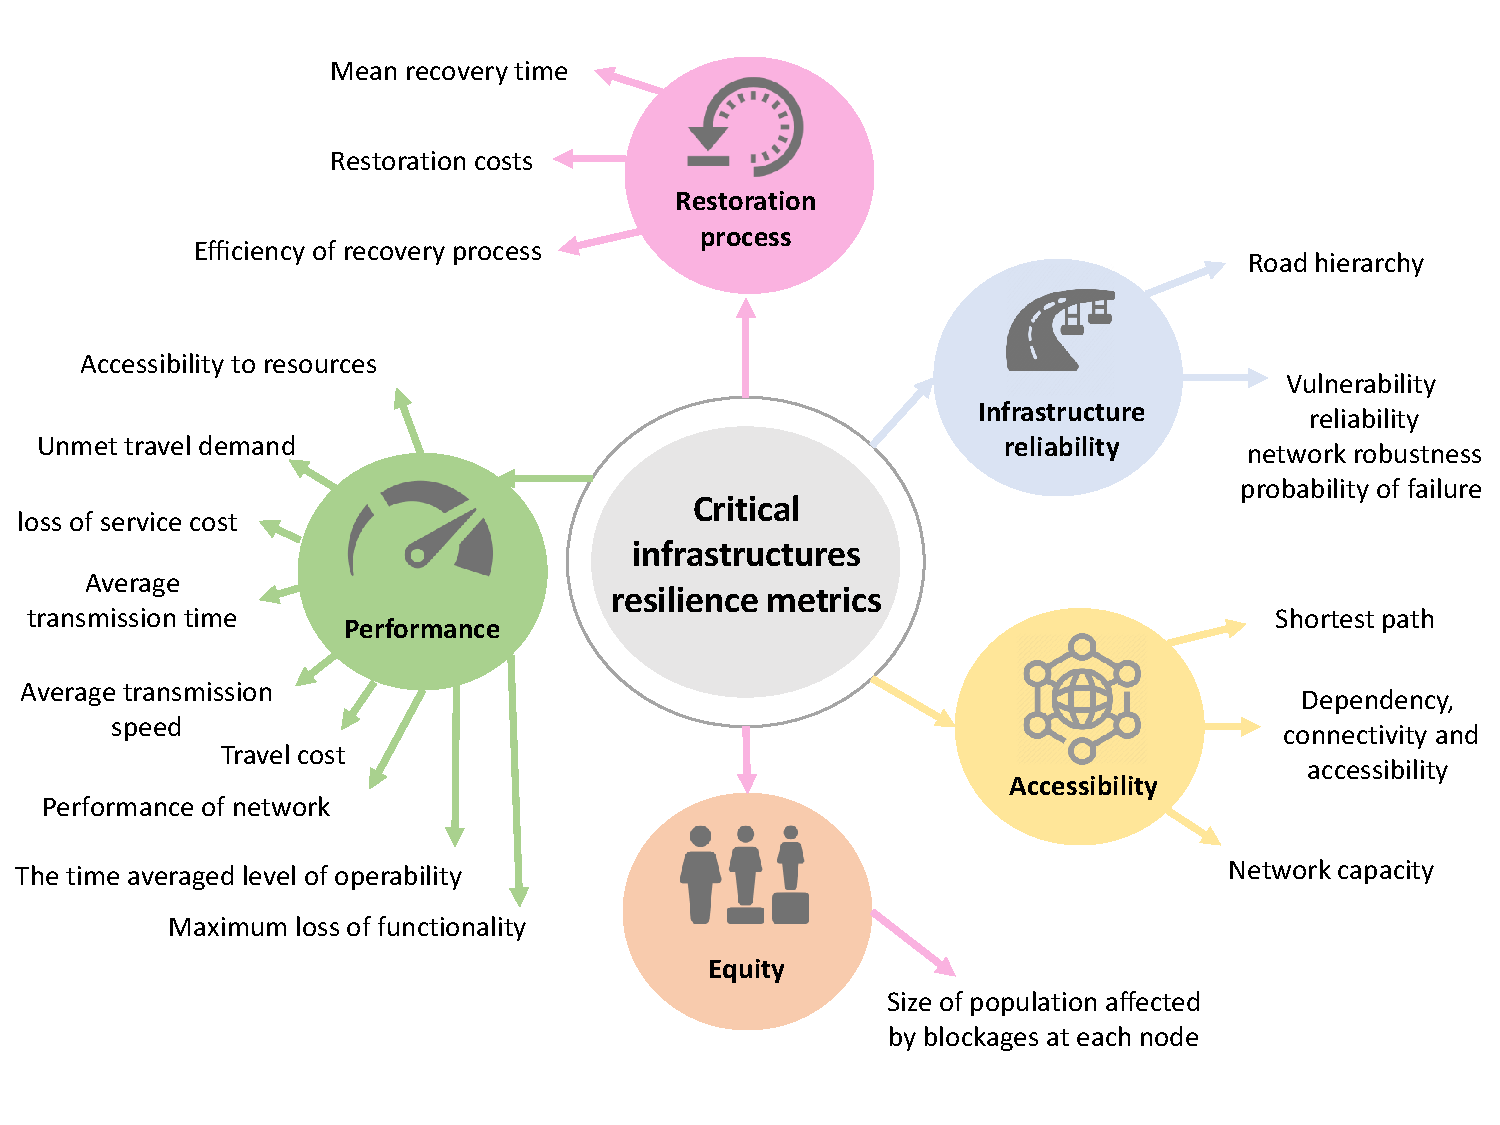
\includegraphics[scale=0.6]{Pic1}
  \caption{Currently used metrics}\label{metric domains}
\end{figure}

\autoref{Table.Overview} provides an overview from all researches which have been reviewed in section 3 and compares them based on applied resilience metrics, case studies, applied method, and provides a brief explanation from their results.\\

\clearpage
\restylefloat{table}
\begin{sidewaystable}[ht]
\scriptsize
\caption{Overview of the researches}
\label{Table.Overview}
\begin{tabular}{>{\raggedright}p{0.09\textwidth} >{\raggedright}p{0.18\textwidth} >{\raggedright}p{0.18\textwidth}
     >{\raggedright}p{0.05\textwidth} >{\raggedright}p{0.05\textwidth} >{\raggedright}p{0.13\textwidth}
   p{0.18\textwidth} }
  \toprule
  \bf Reference & \bf Resilience index & \bf Methods & \bf Multi-layer & \bf Disaster & \bf Case study & \bf Results \\\midrule
  
  Serulle et al (2011) & Road available capacity,
                         Road density,
                         Alternate infrastructure proximity,
                         Level of intermodality,
                         Average delay,
                         Average speed reduction,
                         Personal transport cost, Commercial–industrial transport cost, Network management  &
                                                                                                          Fuzzy logic & No & Flooding
                                                                                      & Santo Domingo, Dominican Republic & Identifying available capacity, alternate infrastructure proximity, and network management as the most important metrics \\
  \midrule
  Antony (2017)         & Centrality measures
                                       & Graph theory analytic & No & natural or man-made disaster & Air and road transportation system of the U.S & Identifying nodes with highest Eigen-vector centrality measures as the most important nodes to restore.\\
  \midrule
  Chen et al(2018) & Vulnerability & Network game theory & No & Man-made emergency events (labor strikes) & China's pre-hinterland container transportation network & Providing behavioral analysis of different players in strategic investment decisions\\
  \midrule
  Aydin et al (2018) & proximity to the main research center, time to recovery  & Topology-based simulation using graph-based connectivity metric of Giant Connected Component(GCC) and Monte Carlo simulation & No & geohazards specially earthquakes & Sindhupalchok District in Nepal & Providing a framework for evaluating road recovery strategies\\
  \midrule
  Bhavathrathan and Patil (2018) & travel time at an upper envelope of operable disruptions & Game theory & No & - & Anaheim city road network & Developing a quantifying resilience framework based on the magnitude of distruptions\\
  \midrule
  Tingting and Yu (2020) & Unmet demand, Total travel time & bi-objective bi-level optimization framework & No & Hurricane, Earthquake, Flood & Road
                                                                                                                                                network in Sioux Falls & Determining optimal resource allocation framework for roadway restoration\\
  \bottomrule
 \end{tabular}
\end{sidewaystable}

% How has uncertainty been handled?
% How do we leverage on computational advances and big data analysis.


\section{Overview of multilayer networks}
Multilayer networks are networks that contain at least two types of nodes or two types of edges
\citep{skrlj2019py3plex}. Multilayer networks are widespread in real world systems such as communication systems, social
systems, transportation systems, and biological systems \citep{wu2020traffic}.  As shown in
\autoref{table.multi-components}, several components can be considered in modeling multilayer networks:

\begin{table}[h!]
  \begin{center}
  \small
  \caption{Multilayer network components}
    \label{table.multi-components}
    \begin{tabular}{p{3in} p{2in}}\toprule
      \textbf{Multilayer network item } & \textbf{References} 
      \\\midrule
      Roads  & \multirow{2}{*}{\citet{antony2017developing}; \citet{zhang2017resiliencebased}} \\
      Bridges &                                \\
      Walkways  & \multirow{2}{*}{\citet{antony2017developing} }\\
      Bike paths  &   \\
      Private roads  &   \\
      High speed and low speed as different layers in a multilayer network & \citet{wu2020traffic} \\
      Public transit & \multirow{2}{*}{\citet{ahmed2020resilience}} \\
      Passenger and freight car transportation systems   &  \\
      Railway & \citet{bhatia2015network} \\\bottomrule
    \end{tabular}
  \end{center}
\end{table}

\subsection{Multilayer modeling of transportation networks}
There are different approaches in modelling transportation networks as a multilayer network.
\citep{wu2020traffic} describes two typical multilayer network models:
\begin{itemize}
  \item Multilayer model with a logical layer and a physical layer
  \item Multilayer model with abstraction of real multilayer networks, in which entities can travel across multiple network layers (for example a high speed layer and a low speed layer)
\end{itemize}
\citet{kurant2006layered} have proposed a generalized multilayer network model in which the lower layer represents the
physical infrastructure and the upper layer represents the traffic flows and applied it to three transportation
systems. This generalized framework facilitates description, comparison and analysis of complex systems such as
transportation networks \citep{kurant2006layered}. \citet{ip2011resilience} have represented transportation networks by
an undirected graph with the nodes as cities and edges as traffic roads and calculated the network resilience of a city
node by the weighted average number of reliable passageways with all other city nodes in the network
\citep{ip2011resilience}. \citet{aleta2017multilayer} have presented a model for representation of the transportation
system of an entire city by considering each line of each mode of transport (bus, metro, and tram) as a single layer and
each stop as a node. Based on their multilayer model, there will be a weighted link (based on distance) between two
nodes on a layer if the corresponding line passes through both of them. They have also added a new layer which
represents the land to introduce the possibility of moving through the city by walking. This model has been applied to
study the interconnected structure of 9 different cities in Europe \citep{aleta2017multilayer}.  \citet{li2019modeling}
have developed an innovative approach in resilience planning of multilayer transportation networks by simulating the
network dynamics of inter-organizational coordination among interdependent infrastructure systems including
transportation, flood control, emergency response, community development, and environmental conservation. They have
examined their model to 35 organizations from five infrastructure systems within Texas, based on the data gathered from
a Hurricane Harvey and evaluated the weaknesses in coordination between entities
\citep{li2019modeling}. \citet{asgari2016ctmapper} proposed an unsupervised mapping algorithm (CT-Mapper) to map sparse
cellular trajectories and modeled a transportation network by a large multilayer graph, in which there are three
different layers of train, subway and road. In this multilayer model, nodes are metro/train stations or road
intersections and edges are connections between them \citep{asgari2016ctmapper}.

\subsection{Multilayer network approaches for critical infrastructure resilience}
\hl{This is where we need to highlight a gap}

\section{Multilayer network model for an equitably resilient system: a conceptual framework}


%\subsection{Expected outcomes}

\section{Conclusion}


\printbibliography

\end{document}

%%% Local Variables:
%%% mode: latex
%%% TeX-master: t
%%% End:
